\\
El algoritmo random forest corresponde a un algoritmo empleado en machine learning registrado por Leo Breiman y Adele Cutler \cite{random-forest}, este combina la salida de múltiples árboles de decisión para llegar a un resultado. El uso de random forest se ha hecho popular a causa de su facilidad de uso y flexibilidad, ya que puede ser empleado para problemas de clasificación y regresión.

El random forest se encuentra formado por varios árboles de decisión, los cuales son propensos a tener problemas como sesgos o sobreajuste, pero cuando se trata con una gran cantidad de árboles se logra llegar a resultados más precisos. ''Mientras que los árboles de decisión consideran todas las posibles divisiones de características, los bosques aleatorios solo seleccionan un subconjunto de esas características.'' \cite{random-forest}

Random forest cuenta con tres hiperparámetros principales que se deben de configurar antes de iniciar el entrenamiento \cite{random-forest}:

\begin{itemize}
    \item Tamaño del nodo.
    \item Cantidad de árboles de decisión.
    \item Cantidad de características muestreadas. 
\end{itemize}

El algoritmo se encuentra compuesto de un conjunto de árboles de decisión, cada árbol del conjunto se encuentra compuesto de una muestra de datos, la cual proviene de un conjunto de entrenamiento con reemplazo, llamada muestra de arranque \cite{random-forest}.

A partir de la muestra de entrenamiento, se extrae un porcentaje para reservarlos como datos de prueba, los cuales se conocen como muestra fuera de la bolsa (oob). Luego, se inyecta otra instancia de aleatoriedad mediante el agrupamiento de características, lo que agrega más diversidad al conjunto de datos y reduce la correlación entre los árboles de decisión \cite{random-forest}.

En un Random Forest, el proceso de predicción puede variar según el tipo de problema que se esté abordando \cite{random-forest}. En el caso de tareas de regresión, se utiliza un enfoque de promediado, donde las predicciones de los árboles de decisión individuales se promedian para obtener el valor final de la predicción. Esto proporciona una estimación más precisa y estable del resultado deseado. Por otro lado, en tareas de clasificación, se utiliza un enfoque de votación mayoritaria. Cada árbol de decisión emite su propia predicción y la clase que obtiene la mayoría de votos se selecciona como la clase predicha. Esto permite tomar una decisión conjunta basada en las opiniones de múltiples árboles, lo que puede mejorar la precisión en la clasificación de las muestras.

Finalmente, la muestra extraída en un comienzo, la muestra fuera de la bolsa (oob) será utilizada para realizar una validación cruzada, finalizando la predicción.

\begin{figure}[H]
    \begin{minipage}[t]{0.9\textwidth}
        \caption{Estructura de un random forest}
        \label{random-forest}        
    \end{minipage}

    \vspace{10pt}

    \begin{minipage}[b]{1.1\textwidth}
        \centering
        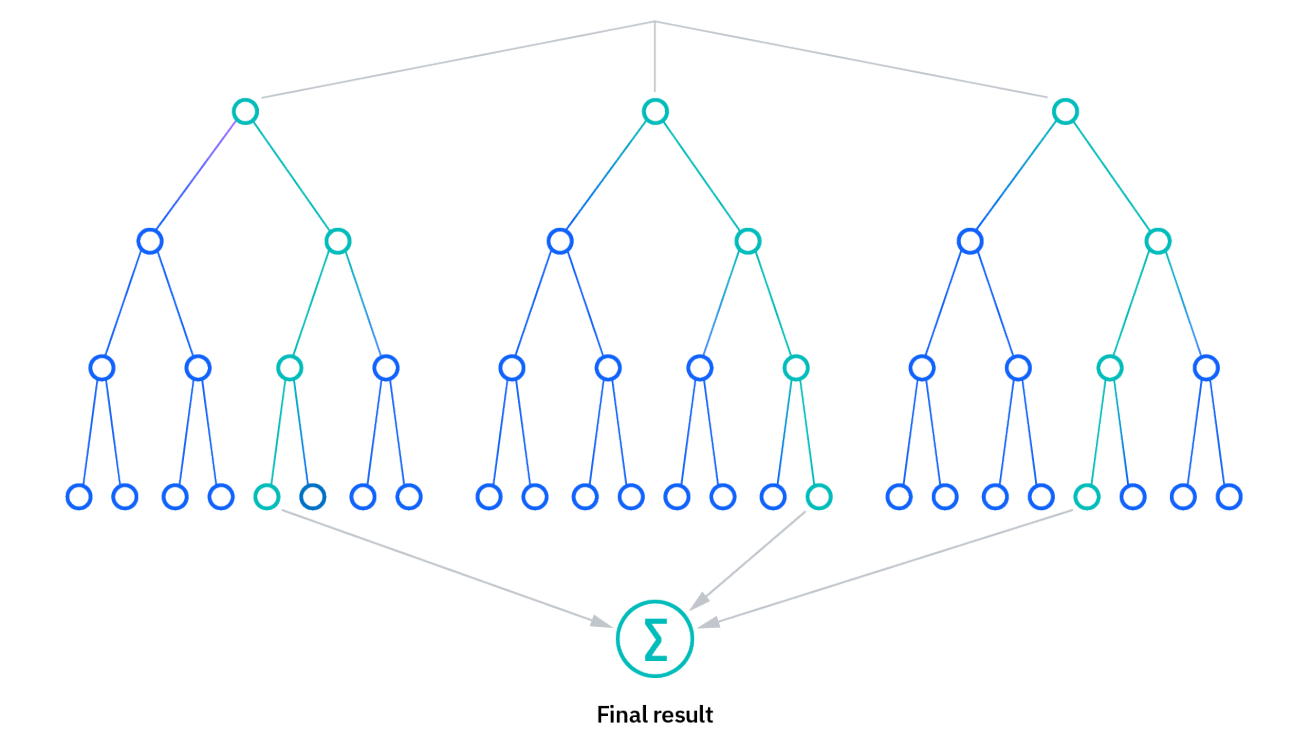
\includegraphics[width=\textwidth]{img/estructura-random-forest.png}        
    \end{minipage}

    \begin{minipage}[t]{0.9\textwidth}
        Fuente: IBM. Recuperado de \url{https://www.ibm.com/mx-es/topics/random-forest}
    \end{minipage}
\end{figure}

\begin{itemize}
    \item \textbf{Ventajas de random forest}
    \begin{itemize}
        \item \textbf{Riesgo reducido de sobreajuste:} Los árboles de decisión corren el riesgo de sobre ajustarse, ya que tienden a ajustar todas las muestras que se encuentran dentro de los datos de entrenamiento. Sin embargo, cuando hay una gran cantidad de árboles de decisión dentro del random forest, el clasificador no será capaz de ajustarse demasiado al modelo, ya que el promedio de los árboles no correlacionados logra reducir la varianza general y el error de predicción.
        \item \textbf{Aporta Flexibilidad:} Debido a su capacidad para abordar con gran precisión tanto tareas de regresión como de clasificación, el método conocido como random forest es ampliamente utilizado por los científicos de datos. Además, su capacidad de agrupar características lo convierte en una herramienta eficaz para estimar valores faltantes, manteniendo la precisión incluso cuando falta parte de los datos.
        \item \textbf{Importancia de la característica fácil de determinar:} El random forest ofrece una forma conveniente de evaluar la importancia o contribución de las variables en un modelo. Existen varias formas de medir la importancia de las características. Por lo general, se utilizan el índice de Gini y la disminución media de impurezas (MDI) para evaluar cuánto afecta la exclusión de una variable específica a la precisión del modelo.
        Sin embargo, otra medida de importancia es la importancia de permutación, también conocida como precisión de disminución media (MDA). La MDA determina la disminución promedio en la precisión al permutar de forma aleatoria los valores de las características en las muestras out-of-bag (muestras que no se utilizan en el proceso de entrenamiento).
    \end{itemize}
    \item \textbf{Desventajas de random forest}
    \begin{itemize}
        \item \textbf{Proceso que requiere mucho tiempo:} Debido a que los algoritmos de random forest son capaces de manejar conjuntos de datos extensos, suelen ofrecer predicciones más precisas. Sin embargo, es importante tener en cuenta que el procesamiento de datos puede volverse lento, ya que se deben calcular los datos para cada árbol de decisión de forma individual.  
        \item \textbf{Requiere más recursos:} Debido a que los random forest procesan conjuntos de datos más grandes, es cierto que se requieren más recursos para almacenar dichos datos. El aumento en el tamaño del conjunto de datos implica una mayor necesidad de memoria y capacidad de almacenamiento para garantizar un funcionamiento eficiente del algoritmo.    
        \item \textbf{Más Complejo:} La interpretación de la predicción de un solo árbol de decisiones resulta más sencilla en comparación con la interpretación de un conjunto de árboles de decisión.
    \end{itemize}
\end{itemize}